\documentclass[10pt,twocolumn]{article}

\usepackage[margin=0.7in,columnsep=0.25in]{geometry}
\usepackage{times}
\usepackage{amsmath,amssymb}
\usepackage{booktabs}
\usepackage{graphicx}
\usepackage{url}
\usepackage[hidelinks]{hyperref}
\usepackage{caption}
\usepackage{hyperref}
\usepackage{enumitem}
\usepackage{tikz}
\usepackage{float}
\usetikzlibrary{arrows.meta, positioning, fit, calc}

\title{Automated Detection of Alzheimer's Disease from Brain MRI Scans}
\author{Alphin Issac Varghese (142401007) \and Aaron C Abraham (142401004)}
\date{}

\begin{document}
\maketitle

\begin{abstract}
    Alzheimer’s disease is a neurodegenerative disease and a common cause of dementia. The symptoms include difficulty in remembering recent events, problems with language, disorientation, mood swings, loss of motivation, self-neglect and behavioral problems.
    Early detection can greatly help in mitigating the effects of this disease. In the early onset of the disease, the cerebrum of the brain tends to shrink due to brain atrophy (Brain cells dying in large numbers). This can be verified via MRI scans of the brain. However this involves having the doctors manually having to see each of about 300-400 brain slices to determine if the patient shows signs of dementia. \\
    In this project we try to use Machine Learning techniques to classify the patients and subsequently we use a Deep Learning based multimodal approach using an extension to the dataset in order to refine the predictions by the model.
\end{abstract}

\section{Introduction}
    \subsection{Dataset Description}
        The dataset used in this project is the \href{https://www.kaggle.com/datasets/ninadaithal/imagesoasis}{OASIS-1 dataset} which has been preprocessed from 3D voxel images to 2D slices, each MRI is converted into 256 z-axis slices in which slices from $100 - 160$ were preserved and the rest were discarded. \\
        A \href{https://www.kaggle.com/datasets/ninadaithal/oasis-1-shinohara/}{supporting dataset} is also used which contains the T1-weighted MRI scans in NIfTI format along with the corresponding metadata. The metadata contains information about the patients such as age, sex, education, socioeconomic status, Mini-Mental State Examination score, estimated total intracranial volume, normalized whole-brain volume, atlas scaling factor and the Clinical Dementia Rating (CDR) which is used as the target variable for classification. \\
        The dataset has approximately 416 subjects with 20 subjects having multiple sessions, for a total of 436 samples. The initial dataset has been used until the mid-term evaluation and the supporting dataset has been used for analysis post the mid-term evaluation

    \subsection{Background Study}
        Alzheimer's disease can be easily observed in the brain MRI scans. The cerebrum of the brain tends to shrink due to brain atrophy and this can be observed in the MRI scans when the CSF volume increases i.e, the white regions in the MRI scans increase. Hence our main goal would be to figure out a way to extract this information via the venticular volume increase and use it to classify the subjects into their appropriate classes.


\section{Data and Preprocessing}
    \begin{center}
        \begin{tabular}{c|c|c|c}
            \toprule
            Class & CDR & Samples & Percentage \\
            \midrule
            Non Demented & 0.0 & 336 & 77.06 \\
            Very mild Dementia & 0.5 & 70 & 16.05 \\
            Mild Dementia & 1.0 & 28 & 6.42 \\
            Moderate Dementia & 2.0 & 2 & 0.46 \\
            \bottomrule
        \end{tabular}
    \end{center}
    
    \noindent
    We observe that the dataset is highly imbalanced with the majority of the samples being non-demented. Hence we will be performing a binary classification task with the following mapping:
    \[
    y =
    \begin{cases}
    0, & \text{Non Demented}\\
    1, & \text{Very Mild, Mild or Moderate Dementia}
    \end{cases}
    \]

    \subsection{\href{https://www.kaggle.com/datasets/ninadaithal/imagesoasis}{2D MRI Slice Dataset}}
         The dataset contains 2D slices of the MRI scans, the following steps were performed for preprocessing the dataset:

         \begin{figure}[H]
            \centering
            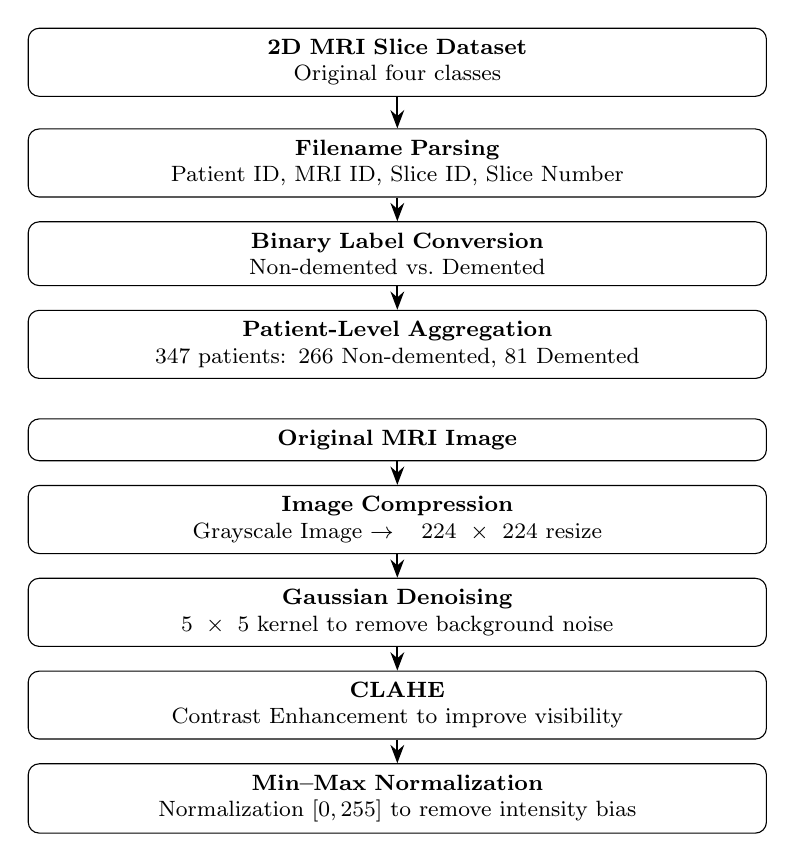
\begin{tikzpicture}[
                node distance=3mm,
                box/.style={
                    draw,
                    rounded corners,
                    align=center,
                    text width=0.75\columnwidth,
                    font=\footnotesize,
                    inner sep=4pt
                },
                smallbox/.style={
                    draw,
                    rounded corners,
                    align=center,
                    text width=0.34\columnwidth,
                    font=\footnotesize,
                    inner sep=4pt
                },
                arrow/.style={
                    -{Stealth},
                    thick
                }
            ]

                \node[box] (input) {
                    \textbf{2D MRI Slice Dataset}\\
                    Original four classes
                };

                \node[box, below=4mm of input] (parse) {
                    \textbf{Filename Parsing}\\
                    Patient ID, MRI ID, Slice ID, Slice Number
                };

                \node[box, below=of parse] (label) {
                    \textbf{Binary Label Conversion}\\
                    Non-demented vs.\ Demented
                };

                \node[box, below=of label] (aggregate) {
                    \textbf{Patient-Level Aggregation}\\
                    347 patients: 266 Non-demented, 81 Demented
                };

                \draw[arrow] (input) -- (parse);
                \draw[arrow] (parse) -- (label);
                \draw[arrow] (label) -- (aggregate);

                \node[box, below = 5mm of aggregate] (preprocess) {
                    \textbf{Original MRI Image}
                };

                \node[box, below = 3mm of preprocess] (gray) {
                    \textbf{Image Compression} \\
                    Grayscale Image 
                    $\rightarrow224\times224$ resize
                };

                \node[box, below = 3mm of gray] (denoise) {
                    \textbf{Gaussian Denoising}\\
                    $5\times5$ kernel to remove background noise
                };

                \node[box, below = 3mm of denoise] (clahe) {
                    \textbf{CLAHE}\\
                    Contrast Enhancement to improve visibility
                };

                \node[box, below = 3mm of clahe] (norm) {
                    \textbf{Min--Max Normalization}\\
                    Normalization $[0,255]$ to remove intensity bias
                };

                \draw[arrow] (preprocess) -- (gray);
                \draw[arrow] (gray) -- (denoise);
                \draw[arrow] (denoise) -- (clahe);
                \draw[arrow] (clahe) -- (norm);

            \end{tikzpicture}
            \caption{2D MRI Image Preprocessing Pipeline.}
            \label{fig:2d_image_aggregation}
        \end{figure}


        \subsection{\href{https://www.kaggle.com/datasets/ninadaithal/oasis-1-shinohara/}{3D MRI NIfTI Dataset}}
        This supporting dataset contains the T1-weighted MRI scans in NIfTI format along with the corresponding metadata which holds the subject level information which will be used for the multimodal approach 

        \noindent
        The following preprocessing steps were performed on the metadata information:
        \begin{figure}[H]
            \centering
            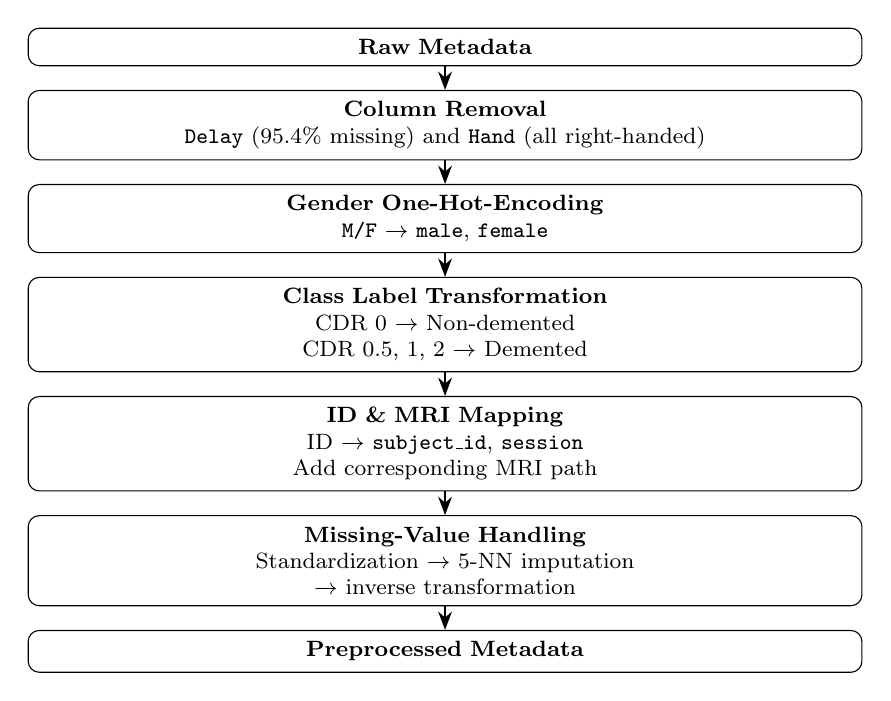
\begin{tikzpicture}[
                node distance=3mm,
                box/.style={
                    draw,
                    rounded corners,
                    align=center,
                    text width=0.85\columnwidth,
                    font=\footnotesize,
                    inner sep=4pt
                },
                arrow/.style={
                    -{Stealth},
                    thick
                }
            ]

                \node[box] (input) {
                    \textbf{Raw Metadata}
                };

                \node[box, below=of input] (remove) {
                    \textbf{Column Removal}\\
                    \texttt{Delay} (95.4\% missing) and
                    \texttt{Hand} (all right-handed)
                };

                \node[box, below=of remove] (gender) {
                    \textbf{Gender One-Hot-Encoding}\\
                    \texttt{M/F} $\rightarrow$ \texttt{male}, \texttt{female}
                };

                \node[box, below=of gender] (target) {
                    \textbf{Class Label Transformation}\\
                    CDR 0 $\rightarrow$ Non-demented\\
                    CDR 0.5, 1, 2 $\rightarrow$ Demented
                };

                \node[box, below=of target] (id) {
                    \textbf{ID \& MRI Mapping}\\
                    ID $\rightarrow$ \texttt{subject\_id}, \texttt{session}\\
                    Add corresponding MRI path
                };

                \node[box, below=of id] (impute) {
                    \textbf{Missing-Value Handling}\\
                    Standardization $\rightarrow$ 5-NN imputation\\
                    $\rightarrow$ inverse transformation
                };

                \node[box, below=of impute] (output) {
                    \textbf{Preprocessed Metadata}
                };

                \draw[arrow] (input) -- (remove);
                \draw[arrow] (remove) -- (gender);
                \draw[arrow] (gender) -- (target);
                \draw[arrow] (target) -- (id);
                \draw[arrow] (id) -- (impute);
                \draw[arrow] (impute) -- (output);

            \end{tikzpicture}
            \caption{Metadata preprocessing pipeline.}
            \label{fig:metadata_preprocessing}
        \end{figure}

        \noindent
        The following preprocessing steps were performed on the 3D MRI voxel information:
        \begin{figure}[H]
            \centering
            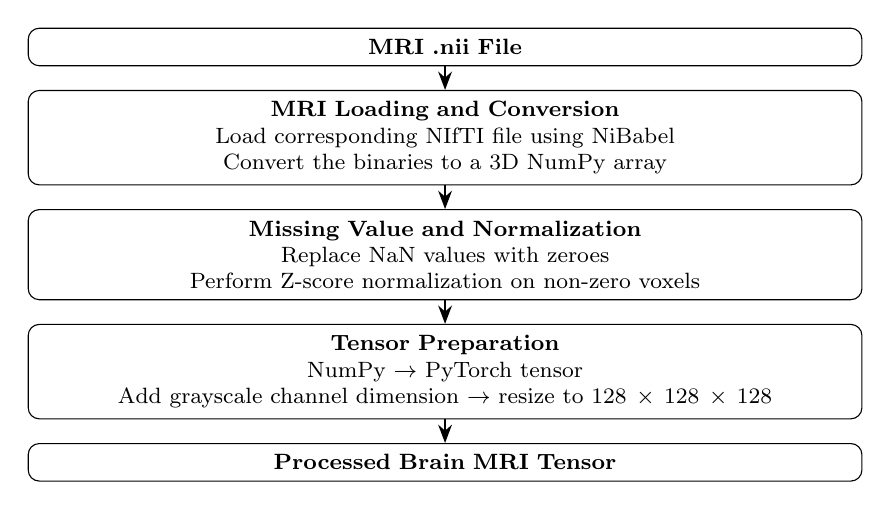
\begin{tikzpicture}[
                node distance=3mm,
                box/.style={
                    draw,
                    rounded corners,
                    align=center,
                    text width=0.85\columnwidth,
                    font=\footnotesize,
                    inner sep=4pt
                },
                arrow/.style={
                    -{Stealth},
                    thick
                }
            ]

                \node[box] (input) {
                    \textbf{MRI .nii File}
                };

                \node[box, below=of input] (load) {
                    \textbf{MRI Loading and Conversion}\\
                    Load corresponding NIfTI file using NiBabel\\
                    Convert the binaries to a 3D NumPy array
                };

                \node[box, below=of load] (clean) {
                    \textbf{Missing Value and Normalization}\\
                    Replace NaN values with zeroes\\
                    Perform Z-score normalization on non-zero voxels
                };

                \node[box, below=of clean] (resize) {
                    \textbf{Tensor Preparation}\\
                    NumPy $\rightarrow$ PyTorch tensor\\
                    Add grayscale channel dimension $\rightarrow$ resize to
                    $128\times128\times128$
                };

                \node[box, below=of resize] (output) {
                    \textbf{Processed Brain MRI Tensor}\\
                };

                \draw[arrow] (input) -- (load);
                \draw[arrow] (load) -- (clean);
                \draw[arrow] (clean) -- (resize);
                \draw[arrow] (resize) -- (output);

            \end{tikzpicture}
            \caption{MRI preprocessing pipeline for the 3D CNN.}
            \label{fig:tensor_preprocessing}
        \end{figure}
        
        \noindent
        The z-score standardisation is performed as follows on voxels $x$ with non-zero mean entires:
        \begin{equation}
            x' = \frac{x-\mu_{nz}}{\sigma_{nz}+10^{-8}},
        \end{equation}
        where $\mu_{nz}$ and $\sigma_{nz}$ are calculated over non-zero voxels. This avoids allowing the background to dominate the intensity statistics.

        \noindent
        The metadata features used for the multimodal approach are summarized in Table~\ref{tab:metadata_features}.
        \begin{table}[htbp]
            \centering
            \begin{tabular}{c|c}
            \toprule
            Feature & Description \\
            \midrule
                ID & Subject and MRI session identifier \\
                Age & Subject's age in years \\
                Sex & Subject's sex (M/F) \\
                Educ & Subject's level of education \\
                SES & Subject's socioeconomic status \\
                MMSE & Mini-Mental State Examination score \\
                eTIV & Estimated total intracranial volume $mm^3$ \\
                nWBV & Normalized whole-brain volume \\
                ASF & Atlas scaling factor \\
                CDR & Clinical Dementia Rating (target variable) \\
            \bottomrule
            \end{tabular}
            \caption{Metadata features used in the multimodal approach.}
            \label{tab:metadata_features}
        \end{table}

\section{Models using 2D Slice Data}
        \subsection{Feature Extraction and Aggregation}
            A set of handcrafted features was extracted from each preprocessed MRI
            slice. The feature extraction pipeline is summarized in Fig.~\ref{fig:feature_pipeline}.

            \begin{figure}[H]
                \centering
                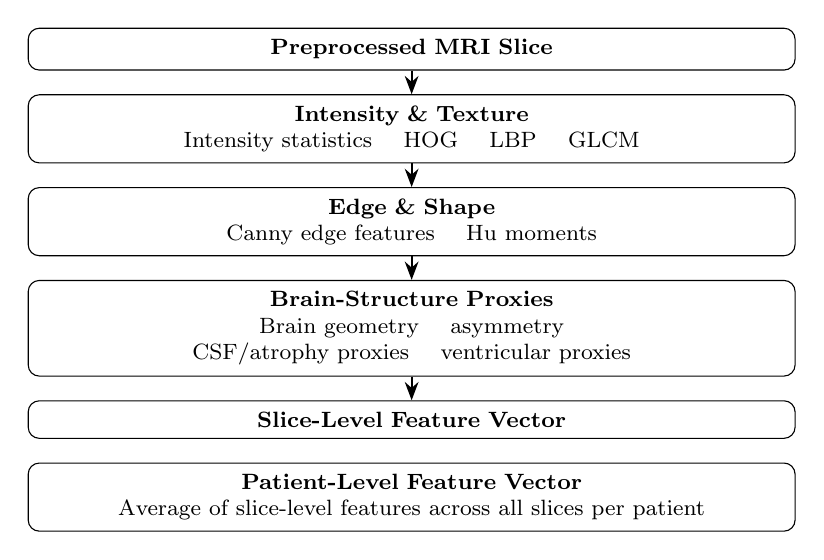
\begin{tikzpicture}[
                    node distance=3mm,
                    box/.style={
                        draw,
                        rounded corners,
                        align=center,
                        text width=0.78\columnwidth,
                        font=\footnotesize,
                        inner sep=4pt
                    },
                    arrow/.style={
                        -{Stealth},
                        thick
                    }
                ]

                    \node[box] (input) {
                        \textbf{Preprocessed MRI Slice}
                    };

                    \node[box, below=of input] (appearance) {
                        \textbf{Intensity \& Texture}\\
                        Intensity statistics \quad HOG \quad LBP \quad GLCM
                    };

                    \node[box, below=of appearance] (shape) {
                        \textbf{Edge \& Shape}\\
                        Canny edge features \quad Hu moments
                    };

                    \node[box, below=of shape] (brain) {
                        \textbf{Brain-Structure Proxies}\\
                        Brain geometry \quad asymmetry \quad
                        CSF/atrophy proxies \quad ventricular proxies
                    };

                    \node[box, below=of brain] (output) {
                        \textbf{Slice-Level Feature Vector}
                    };

                    \node[box, below=of output] (aggregate) {
                        \textbf{Patient-Level Feature Vector}\\
                        Average of slice-level features across all slices per patient
                    };

                    \draw[arrow] (input) -- (appearance);
                    \draw[arrow] (appearance) -- (shape);
                    \draw[arrow] (shape) -- (brain);
                    \draw[arrow] (brain) -- (output);

                \end{tikzpicture}
                \caption{Patient brain feature extraction pipeline.}
                \label{fig:feature_pipeline}
            \end{figure}
        
        \subsection{Model Inferencing and Analysis}
        The feature vectors were standardized and reduced to 10 dims using PCA. The following classifiers were evaluated:

        \noindent
        \begin{tabular}{lccc}
            \toprule
            \textbf{Model} & \textbf{Accuracy} & \textbf{Precision} & \textbf{Recall}\\
            \midrule
            Logistic Regression & 0.686 & 0.369 & 0.453\\
            Random Forest & \textbf{0.729} & 0.375 & \textbf{0.481}\\
            SVC (RBF) & 0.457 & 0.138 & 0.235\\
            KNN & 0.714 & 0.000 & 0.000\\
            Gaussian Naive Bayes & 0.714 & 0.364 & 0.235\\
            MLP & 0.614 & 0.273 & 0.353\\
            Decision Tree & 0.600 & 0.211 & 0.235\\
            \bottomrule
        \end{tabular}

        \noindent
        We observe that in terms of accuracy, the Random Forest model performs the best with an accuracy of 0.729. However, the precision and recall values are low for all models, indicating that the models are not performing well in terms of correctly identifying demented patients.

        \noindent
        This means that simple ML models are unable to capture the complex patterns in the data and hence we will be using a deep learning based approach to improve the performance of the model.

        \noindent
        Subsequently we are only looking at 2D slice data which will not be able to capture the 3D ventricular structures of the brain and hence we will transition to using the 3D MRI data for the deep learning based approach.


\section{Final Classification Framework}
    The final classification framework is a multimodal approach which uses both the 3D MRI data as well as the paitent level metadata information to classify the patients into their respective classes.
    
    \begin{figure}[H]
        \centering
        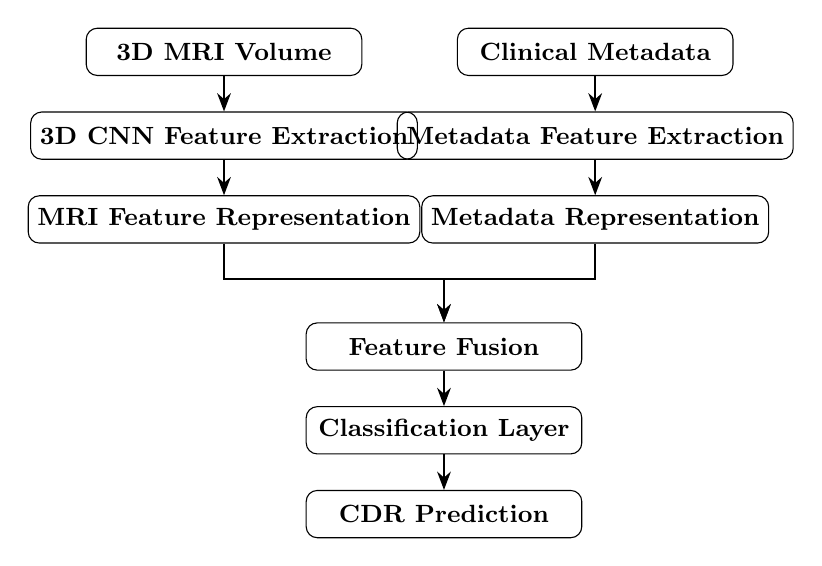
\begin{tikzpicture}[
            node distance=0.45cm,
            box/.style={
                rectangle,
                draw,
                rounded corners,
                minimum width=3.5cm,
                minimum height=0.6cm,
                align=center,
                font=\small
            },
            arrow/.style={
                -{Stealth},
                thick
            }
        ]

            % Left: MRI branch
            \node[box] (mri) {\textbf{3D MRI Volume}};
            \node[box, below=of mri] (cnn) {\textbf{3D CNN Feature Extraction}};
            \node[box, below=of cnn] (mrif) {\textbf{MRI Feature Representation}};

            % Right: Metadata branch
            \node[box, right=1.2cm of mri] (meta) {\textbf{Clinical Metadata}};
            \node[box, below=of meta] (metaf) {\textbf{Metadata Feature Extraction}};
            \node[box, below=of metaf] (metar) {\textbf{Metadata Representation}};

            % Merge
            \node[box, below=1cm of mrif.south east, xshift=0.30cm] (fusion)
                {\textbf{Feature Fusion}};

            \node[box, below=of fusion] (classifier)
                {\textbf{Classification Layer}};

            \node[box, below=of classifier] (output)
                {\textbf{CDR Prediction}};

            % Left branch arrows
            \draw[arrow] (mri) -- (cnn);
            \draw[arrow] (cnn) -- (mrif);

            % Right branch arrows
            \draw[arrow] (meta) -- (metaf);
            \draw[arrow] (metaf) -- (metar);

            % Merge arrows
            \draw[arrow] (mrif.south) -- ++(0,-0.45) -| (fusion.north);
            \draw[arrow] (metar.south) -- ++(0,-0.45) -| (fusion.north);

            % Final arrows
            \draw[arrow] (fusion) -- (classifier);
            \draw[arrow] (classifier) -- (output);

    \end{tikzpicture}
    \caption{Overview of the final multimodal framework.}
    \end{figure}
    


    \subsection{3D CNN Architecture}
       The proposed framework employs a hierarchical 3D convolutional
        architecture to extract spatial features directly from MRI volumes.
        The input is represented as a single-channel 3D tensor and processed
        through four convolutional blocks, with the number of feature channels
        progressively increased from 1 to 128. Each block uses
        $3\times3\times3$ convolutions, followed by batch
        normalisation and ReLU activation. The first three blocks additionally
        apply max pooling to progressively reduce the spatial resolution while
        increasing the abstraction of the learned features.

        \noindent
        The convolutional blocks follow the structure
        \[
        \mathrm{Conv3D}
        \rightarrow
        \mathrm{BatchNorm}
        \rightarrow
        \mathrm{ReLU}
        \rightarrow
        \mathrm{MaxPool},
        \]
        for the first three blocks. The number of channels is as follows:

        \[
        1 \rightarrow 16 \rightarrow 32 \rightarrow 64 \rightarrow 128.
        \]

        \noindent
        The resultingfeature maps are then passed through adaptive average pooling, whichreduces each feature map to a single value. Thus, the resulting representation is transformed as
        \[
        128\times D\times H\times W
        \rightarrow
        128\times1\times1\times1.
        \]
        \noindent
        This produces a fixed-length representation while substantially
        reducing the number of parameters compared with directly connecting
        the feature maps to a fully connected layer.

        \vspace{3pt}
        \noindent
        The pooled representation is flattened and passed through a linear
        layer that projects the 128-dimensional representation to 64
        dimensions. ReLU activation is subsequently applied, followed by
        25\% dropout. The resulting 64-dimensional vector represents the
        learned MRI features and is used as the input to the subsequent
        classification framework.

        \begin{table}[H]
            \centering
            \renewcommand{\arraystretch}{1.15}
            \setlength{\tabcolsep}{4pt}
            \small

            \begin{tabular}{p{1.8cm} p{4.5cm} p{1.55cm}}
                \hline
                \textbf{Stage} & \textbf{Operation} & \textbf{Output} \\
                \hline
                Input
                & 4D MRI volume
                & $1\times128^3$ \\

                Block 1
                & Conv3D + BN + ReLU + MaxPool
                & $16\times64^3$ \\

                Block 2
                & Conv3D + BN + ReLU + MaxPool
                & $32\times32^3$ \\

                Block 3
                & Conv3D + BN + ReLU + MaxPool
                & $64\times16^3$ \\

                Block 4
                & Conv3D + BN + ReLU
                & $128\times16^3$ \\

                Pooling
                & Adaptive Average Pooling
                & $128\times1^3$ \\

                Activation
                & Linear + ReLU + 25\% Dropout
                & $64$ \\

                \hline
            \end{tabular}
        \end{table}
   
    
    \subsection{Metadata Feature Extraction}

\end{document}